%%%%%%%%%%%%%%%%%%%%%%%%%%%%%%%%%%%%%%%%%%%%%%%%%%%%%%%%%%%%%%%%%%%%%%%
%% AGI-22 paper about temporal and procedural reasoning with OpenCog %%
%%%%%%%%%%%%%%%%%%%%%%%%%%%%%%%%%%%%%%%%%%%%%%%%%%%%%%%%%%%%%%%%%%%%%%%

\documentclass[runningheads]{llncs}
%
\usepackage{graphicx}
\usepackage{amsmath}
\usepackage{amssymb}
\usepackage{bussproofs}
\usepackage{cite}

% For ⩘ and ⩗ (requires the LuaLaTeX engine)
\usepackage{unicode-math}
\setmathfont{Stix Two Math}

% Commands for Atomese code
\newcommand{\SP}{\;\;\;}
\newcommand{\TTrue}{\textit{True}}
\newcommand{\TFalse}{\textit{False}}
\newcommand{\TAtom}{\textit{Atom}}
\newcommand{\TTime}{\textit{Time}}
\newcommand{\TEval}{\textit{Evaluation}}
\newcommand{\TList}{\textit{List}}
\newcommand{\TLamb}{\textit{Lambda}}
\newcommand{\TExec}{\textit{Execution}}
\newcommand{\TAtTime}{\textit{AtTime}}
\newcommand{\TAnd}{\textit{And}}
\newcommand{\TOr}{\textit{Or}}
\newcommand{\TNot}{\textit{Not}}
\newcommand{\TImpl}{\textit{Implication}}
\newcommand{\TPredImpl}{\textit{PredictiveImplication}}
\newcommand{\TSeqAnd}{\textit{SequentialAnd}}
\newcommand{\TSeqOr}{\textit{SequentialOr}}
\newcommand{\TBSeqAnd}{\textit{BackSequentialAnd}}
\newcommand{\TFSeqAnd}{\textit{ForeSequentialAnd}}
\newcommand{\TLag}{\textit{Lag}}
\newcommand{\TLead}{\textit{Lead}}
\newcommand{\TTV}{\textit{TV}}
\newcommand{\TTVPi}{\textit{TV}_i^P}
\newcommand{\TTVQi}{\textit{TV}_i^Q}
\newcommand{\TTVP}{\textit{TV}^P}
\newcommand{\TTVQ}{\textit{TV}^Q}
\newcommand{\TTVR}{\textit{TV}^R}
\newcommand{\TTVPQ}{\textit{TV}^{PQ}}
\newcommand{\TTVQR}{\textit{TV}^{QR}}
\newcommand{\TBTV}{\langle \TTV \rangle}
\newcommand{\TBTVPi}{\langle \TTVPi \rangle}
\newcommand{\TBTVQi}{\langle \TTVQi \rangle}
\newcommand{\TBTVP}{\langle \TTVP \rangle}
\newcommand{\TBTVQ}{\langle \TTVQ \rangle}
\newcommand{\TBTVR}{\langle \TTVR \rangle}
\newcommand{\TBTVPQ}{\langle \TTVPQ \rangle}
\newcommand{\TBTVQR}{\langle \TTVQR \rangle}
\newcommand{\Tstrength}{\textit s}
\newcommand{\Tconf}{\textit c}

% Commands for symbolic mathematical notations
\newcommand{\prob}{\mathbf{Pr}}
\newcommand{\limp}{\rightarrow}
\newcommand{\lpreimp}[1]{\leadsto^{#1}}
\newcommand{\lseqor}[1]{\bigslopedvee^{#1}}
\newcommand{\lseqand}[1]{\bigslopedwedge^{#1}}
\newcommand{\ldo}[1]{\widehat{#1}}
\newcommand{\llag}[2]{\overrightarrow{#1}^{#2}}
\newcommand{\llead}[2]{\overleftarrow{#1}^{#2}}
%% TODO: try to replace over right arrow by over right harp, etc
%% \newcommand{\llag}[2]{\accentset{\overrightharp}{#1}^{#2}}
%% \newcommand{\llead}[2]{\overleftharp{#1}^{#2}}

% Commands for schemata vocabulary
\newcommand{\lgo}[1]{\textit{go}(#1)}

\begin{document}
%
\title{Rational OpenCog Controlled Agent}

%\titlerunning{Abbreviated paper title}
% If the paper title is too long for the running head, you can set
% an abbreviated paper title here
%
\author{Nil Geisweiller
  %\orcidID{0000-0001-5041-6299}
  \and Hedra Yusuf}
%
\authorrunning{N. Geisweiller et al.}
% First names are abbreviated in the running head.
% If there are more than two authors, 'et al.' is used.
%
\institute{ SingularityNET Foundation, The
  Netherlands\\ \email{\{nil,hedra\}@singularitynet.io}}
%
\maketitle              % typeset the header of the contribution
%

\begin{abstract}
  TODO
  \keywords{Symbolic Reinforcement Learning \and Procedural Reasoning
    \and OpenCog \and Minecraft}
\end{abstract}

\section{Introduction}

This paper describes an attempt to leverage the OpenCog
framework~\cite{Hart2008} for controlling agents in uncertain
environments.  It can be seen as a reboot of previous
attempts~\cite{Goertzel2008, Goertzel2011, Cai2011, Cai2013} relying
on more mature components such as
\begin{itemize}
\item a hypergraph pattern miner~\cite{Geisweiller2019} and a version
  of PLN~\cite{Goertzel2009} both implemented on top of OpenCog's
  Unified Rule Engine endowed with an inference control mechanism;
\item a temporal and procedural extension of
  PLN~\cite{Geisweiller2023TPLN};
\item a simplified version of OpenPsi~\cite{Cai2011, Cai2013} leaving
  aside built-in urges and modulators from MicroPsi~\cite{Bach2012}
  and using an action selection policy based on Thompson
  Sampling~\cite{Leike2016}.
\end{itemize}
It is comparable to OpenNARS for Applications (ONA)~\cite{Hammer2020}
but, among other differences, uses PLN~\cite{Goertzel2009} as its core
logic rather than NAL~\cite{Wang2011}.

The ultimate goal of this project is to provide a technology to enable
us to experiment with high forms of meta-learning and introspective
reasoning for self-improvements and growth.  The rational for using a
logic-based system is that it offers maximum transparency and is thus
more amenable to reflectivity and introspection~\cite{Schmidhuber2003,
  Goertzel2014EGI1}.  The work that is described in this paper is only
the premise of that goal.  No meta-learning is taking place yet.  The
objective for now is to build an agent that is able to discover its
environment and acts rationally, even at the expense of efficiency.
In a strong sense, the whole system is reasoning-based, from learning
to planning.  The resulting software is called ROCCA for
\emph{Rational OpenCog Controlled Agent}.

% But before to make an agent as rational as possible, not necessarily as
% efficient as possible.  This stems from the concern that in order to
% autonomously gain efficiency the agent must first be able to make the
% best possible decisions, starting first in the outer world, and then
% in the inner world.

% Inner actions could be as transitory as bringing a piece of
% knowledge to the attentional focus, and as profound as rewriting a
% part of its code, like a Goedel Machine.  The atomspace can be
% viewed as a very compact representation of an envelop over
% environments (cite partial operator induction paper).  And PLN can
% be viewed as an abstract-enabling way to calculate the cumulative
% reward (in case it is used as a re-inforcement learner) to be
% maximized, or a goal driven agent in a more general case.  For these
% reasons ROCCA may well be seen as an approximated combination of
% AI\Xi and a Goedel Machine.

% The paper presents

% The agent starts in a completely unknown environment

% The idea is that reasoning is used at all levels, discovering patterns
% from raw observations, building plans and making decisions.

% It is a work in progress.

% Neural networks are excellent at interpolation, but are rather poor at
% extrapolation, what we need for true intelligence is a system that
% thinks critically.

% Rarely do causes and effects take place over arbitrary temporal
% scales.  For instance it is unlikely to find a cause that may produce
% the same effect, or an effect at all, after 1ms, 1 century or any time
% in between.  For that reason we focus on a real time temporal logic.

% \subsection{Related Work}

% ROCCA is essentially a reboot of~\cite{Goertzel2011} using a
% modernized version of the OpenCog pattern miner, as well as a
% simplified version of OpenPsi~\cite{Cai2011, Cai2013} leaving aside
% various built-in urges and modulators from MicroPsi~\cite{Bach2012}
% and using an action selection policy based on Thompson
% Sampling~\cite{Leike2016}.

% \subsection{Contributions}

% The contributions of that paper are:
% \begin{enumerate}
% \item Design an architecture for controlling an agent based on that
%   temporal reasoning extension.
% \end{enumerate}

The rest of the paper is organized as follows.  A recall of the
OpenCog framework is provided in Section~\ref{sec:opencog}.  The ROCCA
software is described in Section~\ref{sec:rocca}.  An experiment using
it to control an agent in Minecraft is described in
Section~\ref{sec:minecraft}.  Finally a conclusion including future
work and directions is given in Section~\ref{sec:conclusion}.
% \subsection{Outline}

% \begin{enumerate}
% \item ROCCA
% \item Minecraft experiment
% \end{enumerate}

\section{OpenCog Framework Recall}
\label{sec:opencog}
OpenCog~\cite{Hart2008} is a framework offering a hypergraph database
technology with a query language and a collection of programs built on
top of it to perform cognitive functions such as learning, reasoning,
spreading attention and more.  Knowledge is stored in
\emph{AtomSpaces}, hypergraphs composed of atoms, links and nodes,
where links can connect to other atoms.  Values can be attached to
atoms to holding probability, confidence, importance and more.  Values
and atoms can be of various types.  Let us recall the types we need
for the rest of paper.
\begin{itemize}
\item A \emph{TruthValue} is a second order probability distribution,
  i.e. the probability of a probability.
\item A \emph{SimpleTrueValue} is a particular TruthValue where the
  second order distribution is represented by a beta distribution of
  parameters controlled by a \emph{strength}, a proxy for a
  probability, and a \emph{confidence} over that probability.  It is
  denoted $<\!s, c\!>$ where $s$ is the strength and $c$ is the
  confidence.
\item A \emph{Predicate} is function from a domain $D$ to $Boolean$.
  A TruthValue can be attached to a predicate, representing the
  prevalence of its satisfied inputs.  For instance
  $P \measeq\ <\!0.4, 0.1\!>$ represents that $P$ tends to evaluate to
  $\textit{True}$ 40\% of the time, but there is a small confidence of
  0.1 over that 40\%.  A TrueValue can be attached to individual
  evaluations as well.  For instance $P(a) \measeq\ <\!0.9, 1\!>$
  represents that the probability of $P(a)$ evaluating to
  $\textit{True}$ is 0.9, and we are certain about it.
\item A \emph{Conjunction} is a link between two predicates,
  representing the predicate resulting from the pointwise conjunction
  of these two predicates.  For instance
  $P \land Q \measeq\ <\!0.2, 0.3\!>$ represents the prevalence, with
  strength 0.2 and confidence 0.3, of the pointwise conjunction of $P$
  and $Q$.
\item An \emph{Implication} is a link between two predicates,
  semantically representing the conditional probability between two
  events represented by these predicates.  For instance
  $P \limp Q \measeq\ <\!0.7, 0.4\!>$ indicates that if $P(x)$ is
  $\textit{True}$ then there is a 70\% change with a 0.4 confidence,
  that $Q(x)$ is also $\textit{True}$.
\end{itemize}
Additionally we use the following types for temporal reasoning.
\begin{itemize}
\item A \emph{Sequential Conjunction} is a link between two temporal
  predicates, representing the predicate resulting from the pointwise
  conjunction of these predicates while the second one is lagging by a
  certain time.  For instance $P \lseqand{T} Q$ is the pointwise
  conjunction of $P$ and a lagging $Q$ by $T$ time units.
\item A \emph{Predictive Implication} is a link between two temporal
  predicates, representing the conditional probability between two
  events lagging by a certain time.  For instance
  $P \lpreimp{T} Q \measeq\ <\!0.8, 0.5\!>$ indicates that if $P(x)$
  is $\textit{True}$ then there is a 80\% chance with a 0.5
  confidence, that after $T$ time units $Q(x)$ will also be
  $\textit{True}$.
\end{itemize}
The difference between a temporal and an atemporal predicate is in its
domain.  The domain of a temporal predicate must have a dimension
respecting certain properties such as having a total order and such.
More detail about the temporal types and their associated inference
rules is provided in~\cite{Geisweiller2023TPLN}.

% that query and modify one or several atomspaces. There is an
% overhaul remaking of OpenCog called Hyperon, but we will not touch
% upon that in that paper as ROCCA is built on top of what we may call
% OpenCog Classic,
% % ~\footnote{OpenCog Classic is still
% %   and will remain in development for the foreseeable future}
% the predecessor of Hyperon.
\section{Rational OpenCog Controlled Agent}
\label{sec:rocca}
\begin{figure}
  \centerline{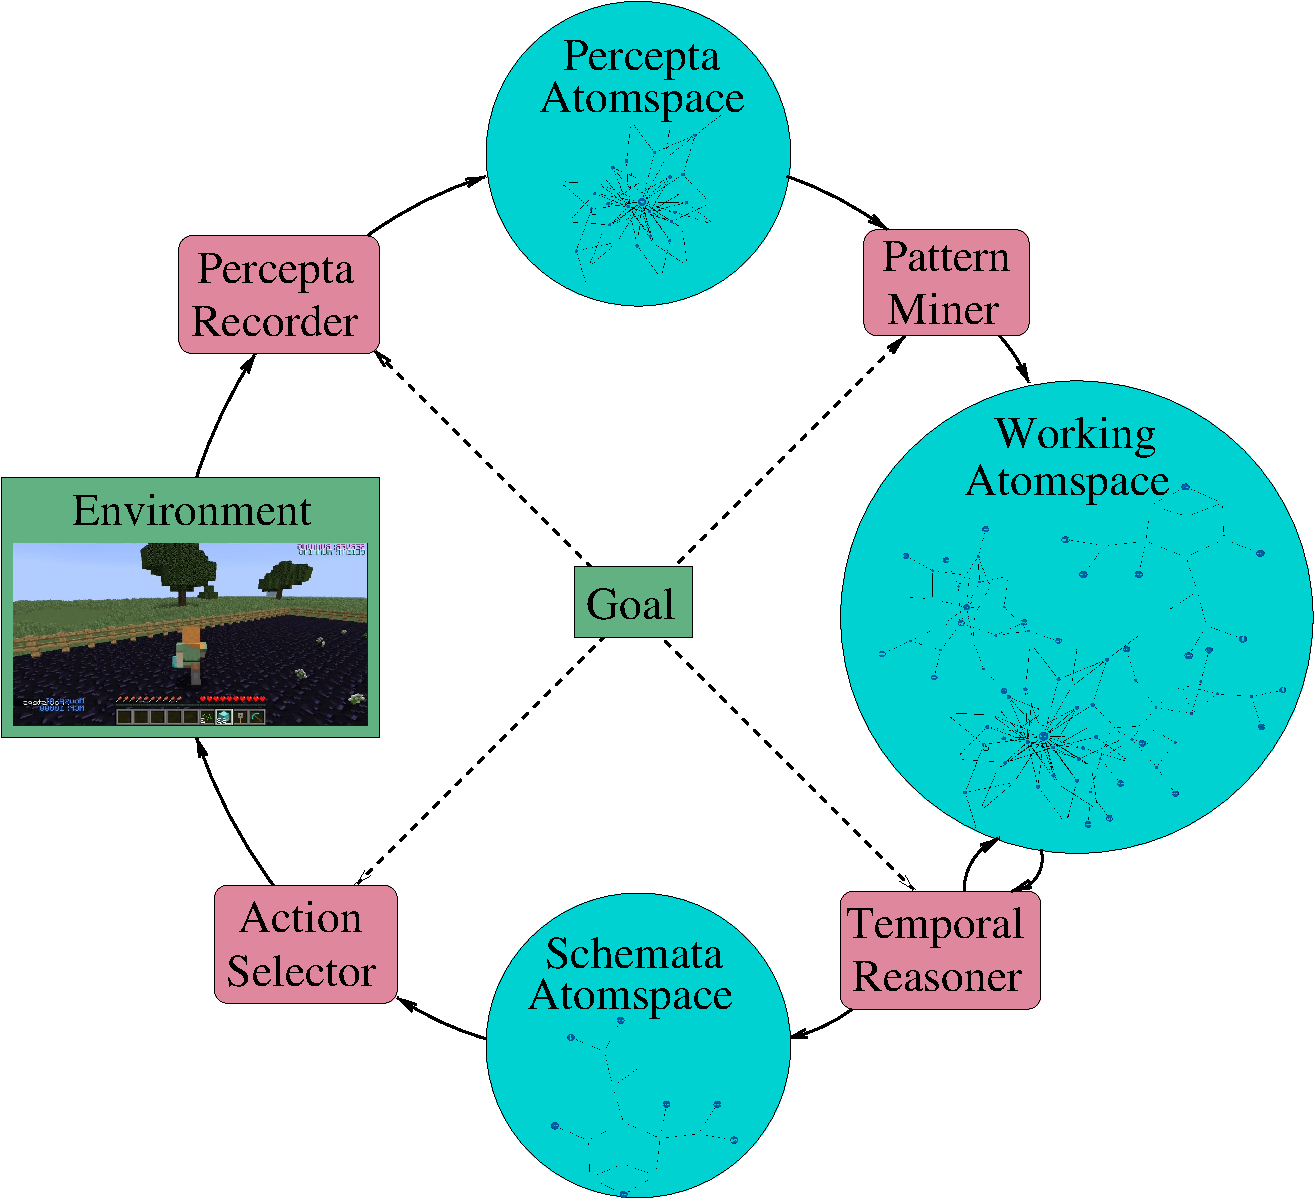
\includegraphics[width=0.6\textwidth]{pictures/rocca-chart-v0.7.pdf}}
  \caption{Rational OpenCog Controlled Agent control and learning
    cycles merged into a single loop}
  \label{fig:rocca}
\end{figure}
To experiment with temporal and procedural reasoning in the context of
embodied virtual agents in unknown environments we have implemented a
project called ROCCA, which stands for \emph{Rational OpenCog
  Controlled Agent}.  ROCCA essentially acts as an interface between
virtual environments such as Malmo \cite{Johnson2016} or OpenAI Gym
\cite{Brockman2016} and OpenCog~\cite{Hart2008}.  It provides an
Observation-Planning-Action control loop as well as various launchers
to run OpenCog processes such as PLN reasoning, pattern mining, etc.
%% During the life of the
%% agent control and learning phases are alternated to simulate a form of
%% online learning.
Provided a top goal, such as maximizing a reward, ROCCA orchestrates
the necessary learning and the planning to fulfill that goal.
%% somewhat like a reinforcement learning agent.
One may possibly see ROCCA as a reinforcement learning agent with the
particularity that learning and planning are, at least in principle,
done via reasoning.
% In that respect it is similar in spirit to
% OpenNARS for Applications (ONA)~\cite{Hammer2020} but uses
% PLN~\cite{Goertzel2009} as its core
% reasoning logic rather than NAL~\cite{Wang2011}.\\
%% Where it differs from a typical
%% reinforcement learning agent in that both learning and planning are,

\subsection{Memory}

The memory of the agent is split into three AtomSpaces:
\begin{enumerate}
\item The \emph{Percepta}\footnote{Percepta means percepts in Latin.
    It is the plurial form of perceptum.  Latin was chosen over
    English so that the difference between singular and plurial does
    not reduce to a single letter, s, which can be prone to error when
    reading and writing code.}  AtomSpace holds timestamped
  observations as they come into the system.
\item The \emph{Working} AtomSpace holds any kind of data, ranging
  from timestamped observations to predictive implications.  Most
  knowledge used and inferred during the course of learning are
  usually dumped into this AtomSpace.
\item The \emph{Schemata} AtomSpace holds predictive implications
  representing cognitive schematics.
\end{enumerate}
The reasons for such splitting are:
\begin{enumerate}
\item Increased \emph{efficiency}, both the Percepta and Schemata
  AtomSpaces are specialized to hold only what is required for rapid
  IO processing.
\item Increased \emph{clarity}, troubleshooting and repairing is
  easier that way.
\end{enumerate}

\subsection{Processes}

Figure~\ref{fig:rocca} shows a large cycle moving through all phases
sequentially.  In theory that is valid, but in practice we want to
split processes, TODO.

ROCCA is composed of two main processes:
\begin{enumerate}
\item \emph{Control} for real-time reactive agent control;
\item \emph{Learning} for non-reactive background learning.
\end{enumerate}

\subsection{Control}
The control process is composed of control cycles, each decomposed
into Observation, Planning and Action phases, described below:
\begin{enumerate}
\item \emph{Observation}:
  \begin{enumerate}
  \item receive and timestamp observations, reward included, from the
    environment,
  \item store the timestamped observations and reward in the Percepta
    AtomSpace.
  \end{enumerate}
\item \emph{Planning}:
  \begin{enumerate}
  \item select the goal for that iteration,
  \item find plans fulfilling that goal from the Schemata AtomSpace,
  \item build a mixture distribution from these plans.
  \end{enumerate}
\item \emph{Action}:
  \begin{enumerate}
  \item select the next action via Thompson Sampling according to that
    mixture distribution,
  \item timestamp and store the selected action in the Percepta
    AtomSpace,
  \item run the selected action and by that update the environment,
  \end{enumerate}
\end{enumerate}
None of these steps are computationally expensive and involve
algorithms that are at most linear with the size of the Percepta and
Schemata AtomSpaces.  For real-time responsiveness however such
control cycle must be temporally bound by a constant.  Achieving this
may entail incorporating other mechanisms such as filtering and
forgetting cognitive schematics.  As important as this problem is
however, it has been let aside for now and is left for future
research.  Given the small environments ROCCA has been tested with, it
has not been a practical problem at this point but will soon be.  More
on the subject of \emph{Attention Allocation} can be found in the
Chapter 4 of~\cite{Goertzel2014EGI2}.

Let us now provide a more detail account of these three phases.

\subsubsection{Observation}
During the observation phase, data coming from the environment are
timestamped and stored in the Percepta AtomSpace.  The format used in
this paper to represent that is \texttt{datum@timestamp}.  For
instance if at cycle 10 the agent observes
\texttt{outside(house)} and
\texttt{hold(key)}, then \texttt{outside(house)@10} and
\texttt{hold(key)@10}
% \begin{itemize}
% \item \texttt{outside(house)}
% \item \texttt{hold(key)}
% \end{itemize}
% then
% \begin{itemize}
% \item \texttt{outside(house)@10}
% \item \texttt{hold(key)@10}
% \end{itemize}
are inserted to the Percepta AtomSpace.

\subsubsection{Planning}

The first step of the planning phase is to select a goal $G$ to
fulfill.  That is an important step that has been elaborated
in~\cite{Goertzel2014EGI1, Hahm2021}.  In the current version of ROCCA
though it merely returns a constant goal which is to gain a reward
within a forward window.  Once a goal has been selected, the agent
queries the Schemata AtomSpace with the following pattern matcher
query
$$\$C \land \$A \lpreimp{T} G$$
where
\begin{itemize}
\item $\$C$ is a variable representing the context,
\item $\$A$ is a variable representing the action or action
  plan~\footnote{Variables are actually typed so that the pattern
    matcher cannot confuse what is context and action.},
\item $T$ is a time delta selected within that forward window,
\item $G$ is a selected goal.
\end{itemize}
All returned candidates are then filtered according to their contexts,
only retaining the ones with contexts being evaluated to true at the
current time.  Ideally a second order probability of a context being
current true would be used, but in the current version of ROCCA a
crisp evaluation is used for the sake of simplicity.

From this set of predictive implications with true contexts, a second
order mixture distribution is built approximating very roughly a
Solomonoff distribution as explained in~\cite{Geisweiller2018}.

\subsubsection{Action}

The Action phase consists of the following steps:
\begin{enumerate}
\item Select the next action via Thompson Sampling according to the
  mixture distribution built during the planning phase.
\item Timestamp and store the selected action in the Percepta
  AtomSpace.
\item Run the selected action and updates the environment.
\end{enumerate}
The trickiest step here is selecting the next action via Thompson
Sampling.  The novelty is that the second order probabilities can be
leveraged by Thompson Sampling.  For example, assume we have two
actions to choose from, $A_1$ and $A_2$, among two predictive
implications
$$
\begin{array}{c}
  C_1 \land A_1 \lpreimp{T} G \measeq\ <\!0.6, 0.9\!> \\
  C_2 \land A_2 \lpreimp{T} G \measeq\ <\!0.7, 0.1\!>
\end{array}
$$
Using only the strengths as proxy for probabilities, the choice is
clear.  Action $A_2$ should be selected, because its probability of
success, which is 0.7, is greater than that of $A_1$, which is 0.6.
However once introducing second order probabilities, that choice
becomes less clear because the truth value of success of $A_2$ has a
low confidence of 0.1.  In that case, first order probabilities are
first sampled from their corresponding second order distributions,
% associated to the truth values of success of $A_1$ and $A_2$,
and then these probabilities are compared.  The action with the
maximum probability wins.  That is the essence of Thompson Sampling.
More informally stated, the idea is to consider the possibilities that
the agent might be living in a world where $A_2$ has a lower
probability of success than $A_1$.
\begin{figure}
  \centerline{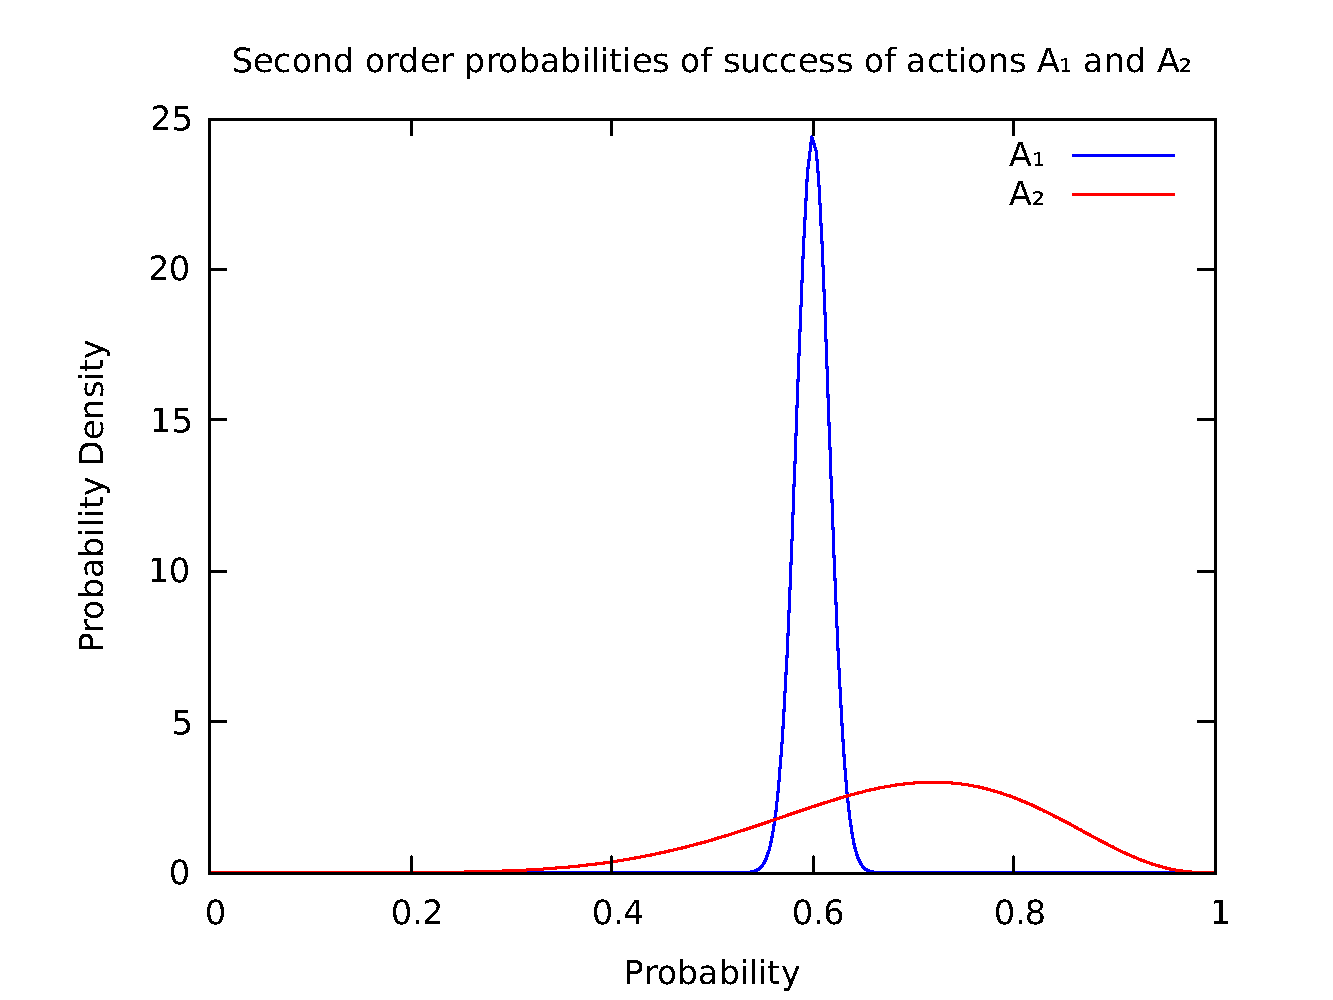
\includegraphics[width=0.8\textwidth]{pictures/actiondist.pdf}}
  \caption{Second order distributions of the probability of success of
    actions $A_1$ and $A_2$, using as parameters of the beta
    distribution $\alpha(s, c)=\alpha_0 + \frac{s.c.K}{1-c}$ and
    $\beta(s, c)=\beta_0 + \frac{(1-s).c.K}{1-c}$} where $K$, the
  \emph{lookahead}, is set to 100, and $\alpha_0$ and $\beta_0$ are
  set to Jeffreys prior.
  \label{fig:actiondist}
\end{figure}
Figure~\ref{fig:actiondist} shows the second order distributions of
the probabilities of success of $A_1$, in blue, and $A_2$, in red, for
these truth values.  As one may notice, the area under the red curve
situated at the left of the blue curve is non-negligible.  Meaning
that the probability of being in a world where $A_1$ has a higher
probability of success than $A_2$ is non-negligible as well.  Because
these strengths and confidences are periodically updated during the
lifetime of the agent, one can see how Thompson Sampling is a great
alternative compared to $\varepsilon$-greedy, offering a
parameter-free mechanism to balance exploration and exploitation that
dynamically adapts with the knowledge of the agent.

Note that in this example above only two actions among two cognitive
schematics are considered, but in practice there usually is a handful
of actions among a potentially very large number of cognitive
schematics, with overlapping, possibly conflicting, contexts and
goals.  The resulting distributions of success of each actions in
those cases are typically multi-modal and do not reduce to beta
distributions.  How to deal with such multitude of cognitive
schematics is treated in~\cite{Geisweiller2018}.

For that we use a variation of Solomonoff induction described
in~\cite{Geisweiller2018} which is especially suited for plans
described by conditional second order distributions, in other words
predictive implications.  More specifically plans are predictive
implication links of the form
$$C \land A \lpreimp{T} G \measeq \textit{TV}$$
called \emph{Cognitive Schematics} or \emph{Schemata}.  Which can be
read as \emph{``in some context $C$, if some action $A$ is executed,
  then after $T$ time units, the goal $G$ is likely to be fulfilled,
  with probability described by $\textit{TV}$''}.  Note that $A$ does
not need to be limited to elementary actions but can be composite as
well, potential describing entire plans composed of action sequences,
conditionals and such, akin to behavior trees.  In other words,
Cognitive Schematics should be expressive enough for general decision
making.
% The likelihood of goal fulfillment is specified by the truth
% value of the predictive implication link, which is not indicated in
% that notational format but is present in the extended Atomese format.
The difficulty then comes down to discovering cognitive schematics
that are as predictive and widely applicable as possible, which
translates into predictive implications which broad contexts, high
strength and high confidence.  An example of an ideal cognitive
schematic would be
$$\mathbb{True} \land A \lpreimp{T} G \measeq\ <\! 1, 1\! >$$
that has a strength and confidence of one, and is universally
applicable\footnote{$\mathbb{True}$ represents the predicate that is
  always true}.  For real environments and goals however, such ideal
is beyond reach.  More often than not we will have instead a large
collection of cognitive schematics with narrow contexts and poor
predictiveness.  To make the best of it, a mixture of second order
distributions is built over all applicable cognitive schematics, in a
manner that approximates a Solomonoff distribution, as described
in~\cite{Geisweiller2018}.  Action selection is then performed based
on that mixture using Thompson Sampling~\cite{Leike2016}.
% , and
% excellent at balancing exploitation and exploration in principle.

\subsection{Learning}
As hinted above, the ultimate goal of the learning phase is to
discover maximally useful cognitive schematics, and by useful it is
specifically meant that they are as predictive and cover as many cases
as possible.

In principle these two processes, Control and Learning, could happen
in parallel.  In practice though, purely for technical simplicity,
they alternate in series.  Basically, the agent starts in a control
phase, a number of control cycles occur as the agent interacts with
its environment, gathers observations and takes (initially random)
actions, which follows then by a long learning phase when the agent
discover regularities in its environments and build plans, and finally
resumes the control phase to test how the agent performs after
learning.

\subsubsection{Pattern Mining}

The advantage of using pattern mining is that already at this stage,
abstract rules can be induced.  For instance the pattern miner can
discover temporal relationships between predicates, such as
$$\lgo{\textit{right}} \lpreimp{1} square(right)$$
$$go(left) \lpreimp{1} square(left)$$
meaning that if the agent goes to the right (resp. left), at the next
time unit, it will be located on the right (resp. left) square.  But
it can also discover abstractions such as
$$\lgo{x} \lpreimp{1} square(x)$$
The pattern mining algorithm used in ROCCA is actually a specialized
form of reasoning, that is easily interlaced with more general forms
of reasoning~\cite{Geisweiller2019}.

As it stands, pattern mining can be a relatively inexpensive way to
generate mono-action cognitive schematics.  Mining poly-action
cognitive schematics is possible but has two drawbacks:
\begin{enumerate}
\item In the worse case, the computational cost of mining goes up
  exponentially with the size of the action sequence to mine.
\item The number of observations to accumulate in order to generate
  cognitive schematics with decent confidences goes up exponentially
  as well.
\end{enumerate}
The latter is really the most limiting factor because we cannot buy
our way out of it.  If each observation takes a certain amount time,
determined by the control cycle period in the case of primary
observations, then we have to do through them, we cannot speed time
up.  This is even more true for abstract percepts that can only be
observed at periods which are multiples of control cycle periods.
Also, in some cases, a particular action sequence may even never be
observed at all, yet we still would like to have a way to estimate the
likelihood of its success.  In order to address these limitations, and
to build complex cognitive schematics with good probability estimates
and confidences, we need reasoning.

\subsubsection{Temporal and Procedural Reasoning}

ROCCA uses a temporal extension of PLN, described in detail
in~\cite{Geisweiller2023TPLN}, to infer new cognitive schematics, not
only from direct observations, or also based on other cognitive
schematics and background knowledge.  An example would be to combine
mono-action plans to infer poly-action plans.  Another example would
be to specialize a context or a goal.  As for now three temporal rules
are integrated into ROCCA:

\begin{enumerate}
\item Predictive Implication Direct Introduction: TODO.
\item Temporal Conditional Conjunction Introduction: TODO.
\item Temporal Deduction: TODO.
\end{enumerate}

The precise semantics of these rules is detailed
in~\cite{Geisweiller2023TPLN}.  An example of how these rules are used
in ROCCA is detailed in Section~\ref{sec:minecraft}.

\section{Experiment with Simple Minecraft Environment}
\label{sec:minecraft}
In this experiment we built a minecraft environment using Malmo, which is a platform for Artificial Intelligence experimentation and research built on top of Minecraft. The demo environment consists of a small house with a locked door, diamonds inside and a key to get into the house. The agent, initially located outside of the house, can perform different actions like getting a key, opening a door of the house and collecting the diamonds in order to achieve a reward. \par
The aim of this experiment is to make the ROCCA agent learn from the actions and perceptions in the minecraft environment and do efficient planning so as to be able to collect as many diamonds as possible and accumulate reward. The ROCCA agent will be able to perform a series of possible actions with a goal of achieving a reward and learns from them by applying PLN (Probabilistic Logic Networks) and Pattern Miner, which can be seen as a specialized form of PLN reasoning. The Planning, the discovery of cognitive schematics, is also handled by PLN and its temporal reasoning rule base.

\begin{figure}[htbp]
\centerline{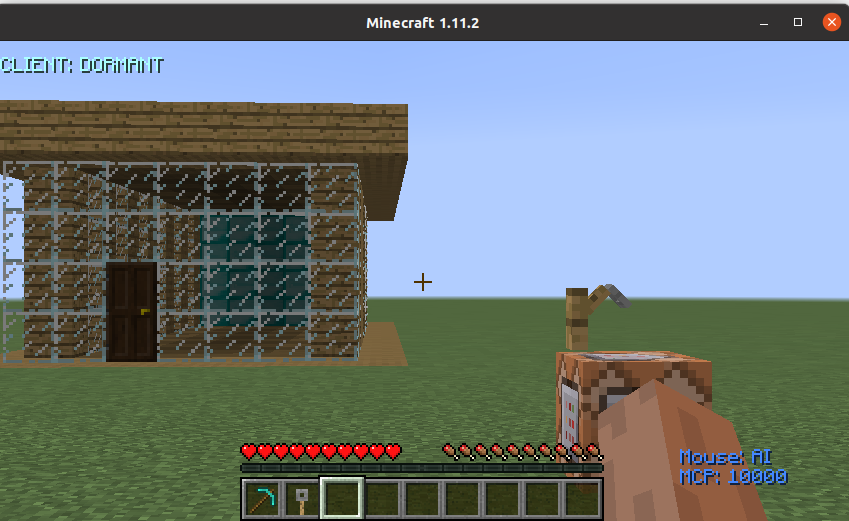
\includegraphics[scale=.2]{pictures/simple_demo.png}}
\caption{Simple Minecraft demo with a house and a key.}
\label{fig:minecraft}
\end{figure}

There are lists of allowed actions provided by minecraft that an agent can perform like moving, turning, picking etc.. but due to the limited processing capacity we have to handle the observations from each action and to reduce complexity, we proposed to have an abstract action and perception where unnecessary details have been omitted. With that we generate three abstract actions namely go-to-key, go-to-house, go-to-diamonds where each of them contains a series of actions and returns an abstract perception about where the agent is (inside house, outside house, next to closed door etc..), about its inventory (has key, diamond pickaxe etc..) and the reward of completing a given action. \par
We perform various experiments tuning different parameters. A typical experiment has two iterations of the learning-training process with a duration of fifty iterations for each training. In the first cycle the agent will not have prior knowledge hence no learning will take place. The agent pursues the environment and builds its knowledge base by trying a combination of fifty randomly weighted actions. At the end of the first cycle the agent will have enough background knowledge to apply Pattern miner and PLN temporal reasoning. Hence, during the second cycle, the agent will be able to learn and plan the desired cognitive schematics which leads to a positive goal of getting a reward.\\
The ROCCA agent is able to learn the following cognitive schematics with higher strength.

$$\textit{outside}(\textit{self}, \textit{house}) \land \ldo{\textit{go\_to}(\textit{key})} \lpreimp{1} \textit{hold}(\textit{self}, \textit{key})$$
$$\textit{hold}(\textit{self}, \textit{key}) \land \ldo{\textit{go\_to}(\textit{house})} \lpreimp{1} \textit{inside}(\textit{self}, \textit{house})$$
$$\textit{inside}(\textit{self}, \textit{house}) \land \ldo{\textit{go\_to}(\textit{diamond})} \lpreimp{1} \textit{reward}(1)$$

In this experiment, we measure the agent's performance by the cognitive schematics learned and accumulated rewards achieved. The ROCAA agent is successful in learning the required cognitive schematics which leads the agent to collect more rewards in the second cycle. However, these findings with a simple minecraft environment with only few actions might not tell the overall performance of ROCCA. As a future work, further extensive experiments are needed to conclude the performance achieved.

\section{Conclusion}
\label{sec:conclusion}
We have introduced an agent called ROCCA that leverages the OpenCog
framework for controlling an agent in unknown and uncertain
environments.  ROCCA is meant to be as rationally as possible, at the
expense of efficiency when needed.  For now it is only able to operate
is very simple environments involving a handful of actions and
observations.  The type of learning used is however meant be
open-ended, even though for now it is limited to syntactic hypergraph
pattern mining and other limited form of temporal reasoning.  As of
now it is able to build mine small plan from direct observations and
larger plans from smaller plans using probabilistic reasoning.

This is a preparatory work of a greater goal, which is to explore
deeper forms of meta-learning and introspective reasoning.  Towards
that end the remaining milestones are:
\begin{enumerate}
\item Support temporal intervals and scales and add more temporal, as
  well as spatial inference rules.
\item Integrate ECAN~\cite{TODO} for \emph{Attention Allocation}, as
  well as record attention spreading to learn Hebbian links and
  improve attention allocation.
\item Carry out concept creation and schematization, also called
  crystallized attention allocation, to speed up repetitive
  information processing even further.  It should be noted that this
  done well should also provide a solution for the problem of creating
  abstract observations and actions.
\item Record more internal processes, not just attention spreading, as
  internal percepta to enable deeper forms of introspection.
\item Plan internal actions, not just external, to enable self-growth.
\end{enumerate}

% \begin{enumerate}
% \item Forgetting
% \item Functional Pattern Mining
% \item Attention Allocation
% \item Inner actions
% \item Port to OpenCog Hyperon
% \item Higher level percepts
% \item Second order evaluation of context being currently true
% \item Time interval
% \end{enumerate}

%
% ---- Bibliography ----
%
\bibliographystyle{splncs04} \bibliography{local}

\end{document}
